\documentclass{article}
\usepackage[utf8]{inputenc}
\usepackage{tikz}
\usepackage[left=2cm,right=2cm,top=2cm,bottom=2cm]{geometry}

\usetikzlibrary{shapes.geometric, arrows}

\title{Game Doc}
\author{Gaël Berthaud-Müller}
\date{June 2018}


\tikzstyle{startstop} = [rectangle, rounded corners, minimum width=3cm, minimum height=1cm,text centered, draw=black]
\tikzstyle{io} = [trapezium, trapezium left angle=70, trapezium right angle=110, minimum width=3cm, minimum height=1cm, text centered, draw=black, text width=3cm]
\tikzstyle{process} = [rectangle, minimum width=3cm, minimum height=1cm, text centered, draw=black, text width=3cm]
\tikzstyle{decision} = [diamond, minimum width=3cm, minimum height=1cm, text centered, draw=black, aspect=2, text width=3cm]

\tikzstyle{arrow} = [thick,->,>=stealth]
\tikzstyle{arrow} = [thick,->,>=stealth,]
\tikzstyle{line} = [thick,-]


\begin{document}

\maketitle
\tableofcontents
\newpage
\section{Think functions}

All the game logic is done by what we are going to call \textit{think functions}. A think function is a single function that is responsible of a certain task. That task should be atomic if possible.
Think function can be triggered by different ways, on action, loop or event. In this document those types are reffered as \textit{@on\_action}, \textit{@on\_loop}, \textit{@on\_event}.

The first one happens when a new action occures, either emitted by the local peer or a distant one. A \textit{@on\_action} think function take as arguments the type of action and the parametters of that action.

Next we have the \textit{@on\_loop} think function that will be executed at each loop iteration. To guarantee the atomicity of the think function it can be restrained to a specific entity. The function will then be called once for each object that is managed by the current peer with that object passed as argument.

At last, the \textit{@on\_event} think function is used as an handler for system event.
\section{Peers Management}
\subsection{Join process}

\begin{minipage}{0.6\textwidth}\centering
  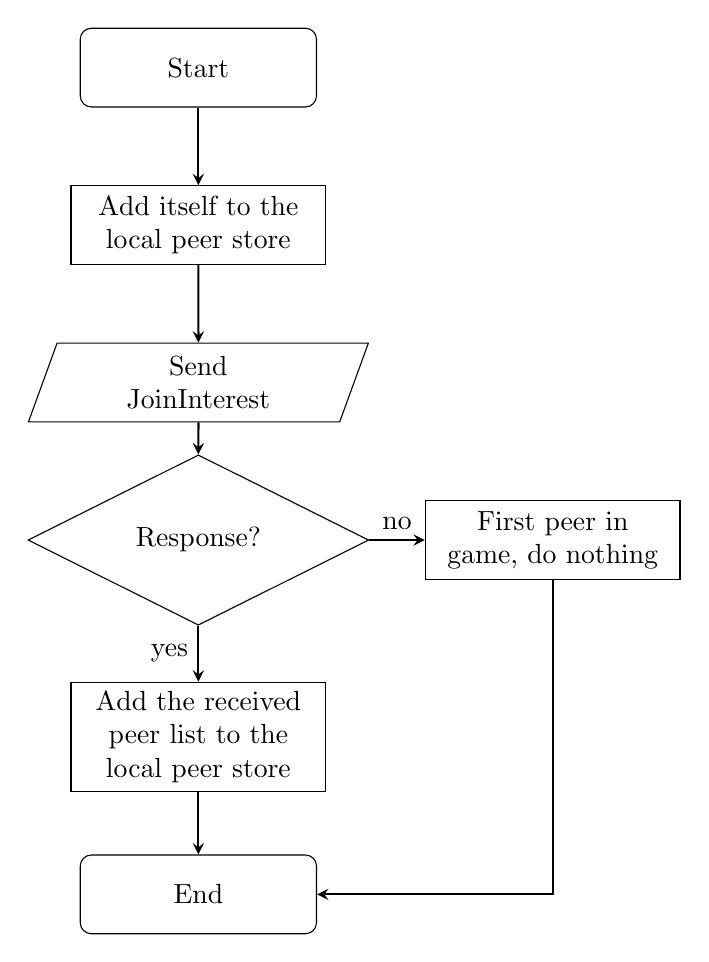
\begin{tikzpicture}[node distance=2cm]
    \node (start) [startstop] {Start};
    \node (pro3) [process, below of=start] {Add itself to the local peer store};
    \node (out1) [io, below of=pro3] {Send \\ JoinInterest};
    \node (dec1) [decision, below of=out1] {Response?};
    \node (pro1) [process, below of=dec1, yshift=-0.5cm] {Add the received peer list to the local peer store};
    \node (pro2) [process, right of=dec1, xshift=2.5cm] {First peer in game, do nothing};
    \node (stop) [startstop, below of=pro1] {End};

    \draw [arrow] (start) -- (pro3);
    \draw [arrow] (pro3) -- (out1);
    \draw [arrow] (out1) -- (dec1);
    \draw [arrow] (dec1) -- node[anchor=east] {yes} (pro1);
    \draw [arrow] (dec1) -- node[anchor=south] {no} (pro2);
    \draw [arrow] (pro1) -- (stop);
    \draw [arrow] (pro2) |- (stop);
  \end{tikzpicture}
\end{minipage}
\begin{minipage}{0.4\textwidth}\centering
  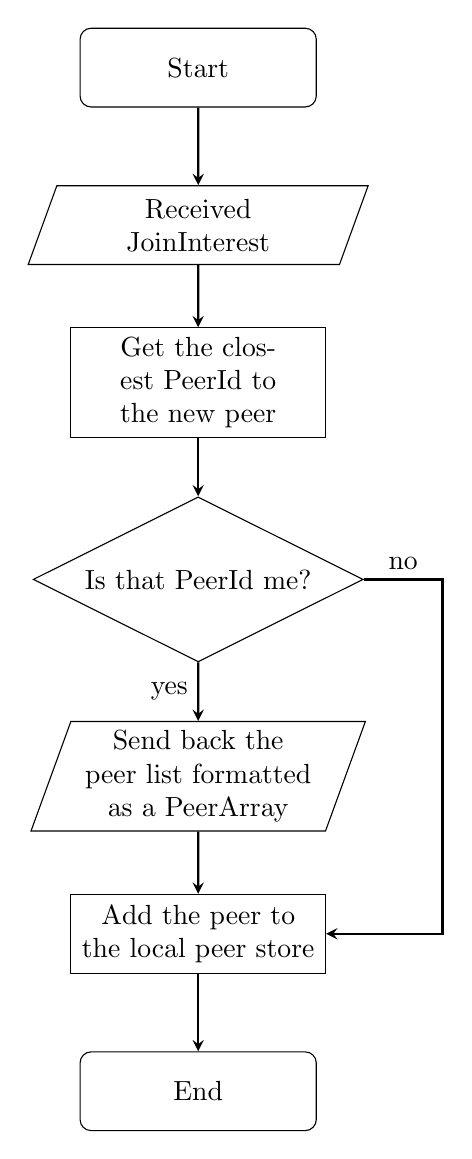
\begin{tikzpicture}[node distance=2cm]

    \node (start) [startstop] {Start};
    \node (in1) [io, below of=start] {Received JoinInterest};
    \node (pro1) [process, below of=in1] {Get the closest PeerId to the new peer};
    \node (dec1) [decision, below of=pro1, yshift=-0.5cm] {Is that PeerId me?};
    \node (out1) [io, below of=dec1, yshift=-0.5cm] {Send back the peer list formatted as a PeerArray};
    \node (pro2) [process, below of=out1] {Add the peer to the local peer store};
    \node (stop) [startstop, below of=pro2] {End};

    \draw [arrow] (start) -- (in1);
    \draw [arrow] (in1) -- (pro1);
    \draw [arrow] (pro1) -- (dec1);
    \draw [arrow] (dec1) -- node[anchor=east] {yes} (out1);
    \draw [arrow] (dec1.east) -- node[anchor=south] {no} ++ (1,0) |- (pro2.east);
    \draw [arrow] (out1) -- (pro2);
    \draw [arrow] (pro2) -- (stop);

  \end{tikzpicture}
\end{minipage}

\subsection{Leave process}
\begin{minipage}{0.5\textwidth}\centering
  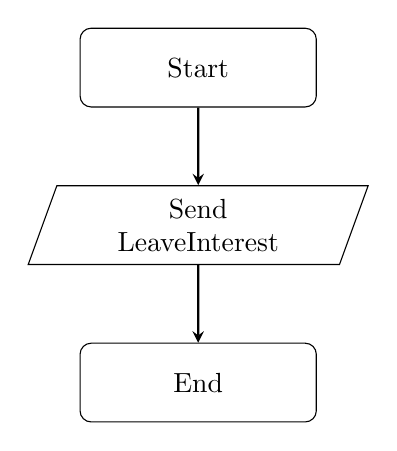
\begin{tikzpicture}[node distance=2cm]
    \node (start) [startstop] {Start};
    \node (out1) [io, below of=start] {Send\\ LeaveInterest};
    \node (stop) [startstop, below of=out1] {End};

    \draw [arrow] (start) -- (out1);
    \draw [arrow] (out1) -- (stop);
  \end{tikzpicture}
\end{minipage}
\begin{minipage}{0.5\textwidth}\centering
  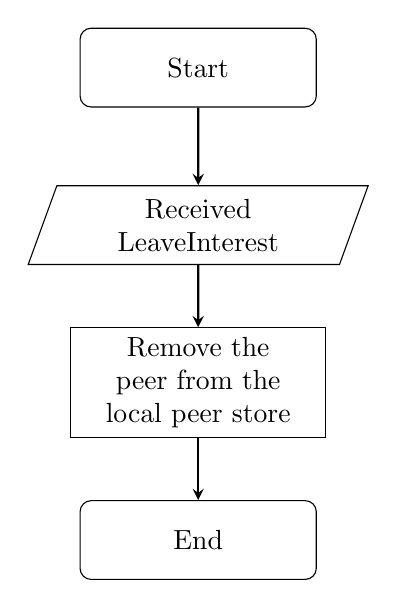
\begin{tikzpicture}[node distance=2cm]
    \node (start) [startstop] {Start};
    \node (in1) [io, below of=start] {Received LeaveInterest};
    \node (pro1) [process, below of=in1] {Remove the peer from the local peer store};
    \node (stop) [startstop, below of=pro1] {End};

    \draw [arrow] (start) -- (in1);
    \draw [arrow] (in1) -- (pro1);
    \draw [arrow] (pro1) -- (stop);
  \end{tikzpicture}
\end{minipage}

\section{Objects Management}
\subsection{From players}
\subsubsection{Global process}

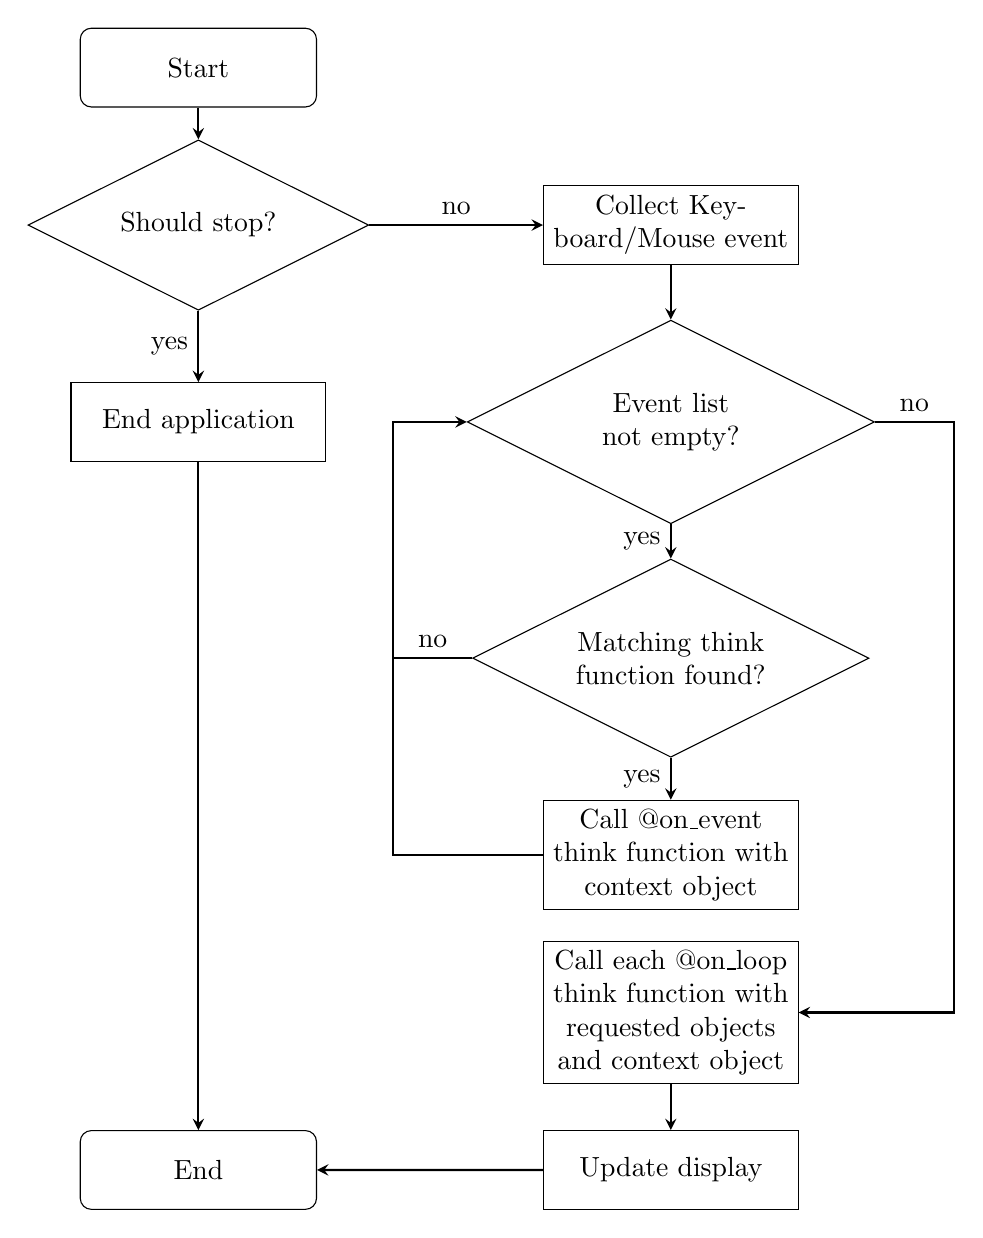
\begin{tikzpicture}[node distance=2cm]
  \node (start) [startstop] {Start};
  \node (dec1) [decision, below of=start] {Should stop?};
  \node (pro1) [process, right of=dec1, xshift=4cm] {Collect Keyboard/Mouse event};
  \node (dec2) [decision, below of=pro1, yshift=-0.5cm] {Event list not empty?};
  \node (dec3) [decision, below of=dec2, yshift=-1cm] {Matching think function found?};
  \node (pro2) [process, below of=dec3, yshift=-0.5cm] {Call @on\_event think function with context object};
  \node (pro3) [process, below of=pro2] {Call each @on\_loop think function with requested objects and context object};
  \node (pro4) [process, below of=pro3] {Update display};
  \node (pro5) [process, below of=dec1, yshift=-0.5cm] {End application};
  \node (stop) [startstop, below of=pro5, yshift=-7.5cm] {End};

  \draw [arrow] (start) -- (dec1);
  \draw [arrow] (dec1) -- node[anchor=east] {yes} (pro5);
  \draw [arrow] (pro5) -- (stop);
  \draw [arrow] (dec1) -- node[anchor=south] {no} (pro1);
  \draw [arrow] (pro1) -- (dec2);
  \draw [arrow] (dec2) -- node[anchor=east] {yes} (dec3);
  \draw [arrow] (dec3) -- node[anchor=east] {yes} (pro2);
  \draw [arrow] (pro3) -- (pro4);
  \draw [arrow] (pro4) -- (stop);

  \draw [arrow] (dec2.east) -- node[anchor=south] {no} ++ (1,0) |- (pro3.east);
  \draw [arrow] (dec3.west) -- node[anchor=south] {no} ++ (-1,0) coordinate (aux) |-  (dec2.west);
  \draw [line] (pro2.west) -| (aux);

\end{tikzpicture}

\subsubsection{Fetching objects}

\subsubsection{Getting updates}

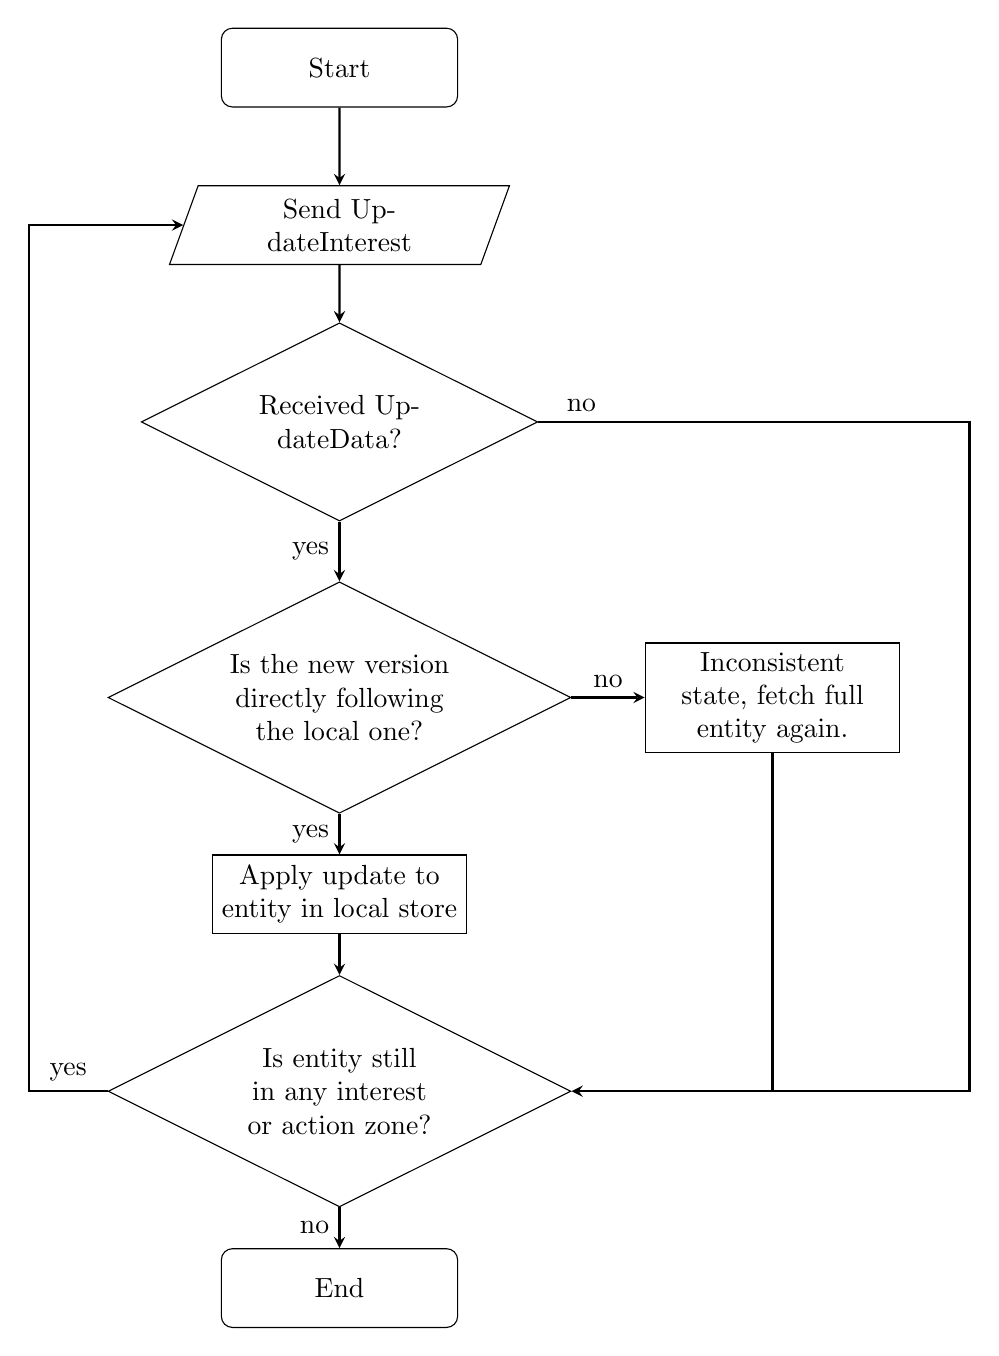
\begin{tikzpicture}[node distance=2cm]
  \node (start) [startstop] {Start};
  \node (out1) [io, below of=start] {Send UpdateInterest};
  \node (dec1) [decision, below of=out1, yshift=-0.5cm] {Received UpdateData?};
  \node (dec2) [decision, below of=dec1, yshift=-1.5cm] {Is the new version directly following the local one?};
  \node (pro1) [process, below of=dec2, yshift=-0.5cm] {Apply update to entity in local store};
  \node (dec3) [decision, below of=pro1, yshift=-0.5cm] {Is entity still in any interest or action zone?};
  \node (stop) [startstop, below of=dec3, yshift=-0.5cm] {End};
  \node (pro2) [process, right of=dec2, xshift=3.5cm] {Inconsistent state, fetch full entity again.};

  \draw [arrow] (start) -- (out1);
  \draw [arrow] (out1) -- (dec1);
  \draw [arrow] (dec1) -- node[anchor=east] {yes} (dec2);
  \draw [arrow] (dec2) --  node[anchor=east] {yes} (pro1);
  \draw [arrow] (pro1) -- (dec3);
  \draw [arrow] (dec3) -- node[anchor=east] {no} (stop);
  \draw [arrow] (dec3.west) -- node[anchor=south] {yes} ++ (-1,0) |-  (out1.west);
  \draw [arrow] (dec2) -- node[anchor=south] {no} (pro2);
  \draw [arrow] (pro2) |- coordinate (aux) (dec3);
  \draw [line] (dec1) -- node[anchor=south,pos=0.1] {no} ++ (8,0) |- (aux);
\end{tikzpicture}

\subsubsection{Emitting actions}

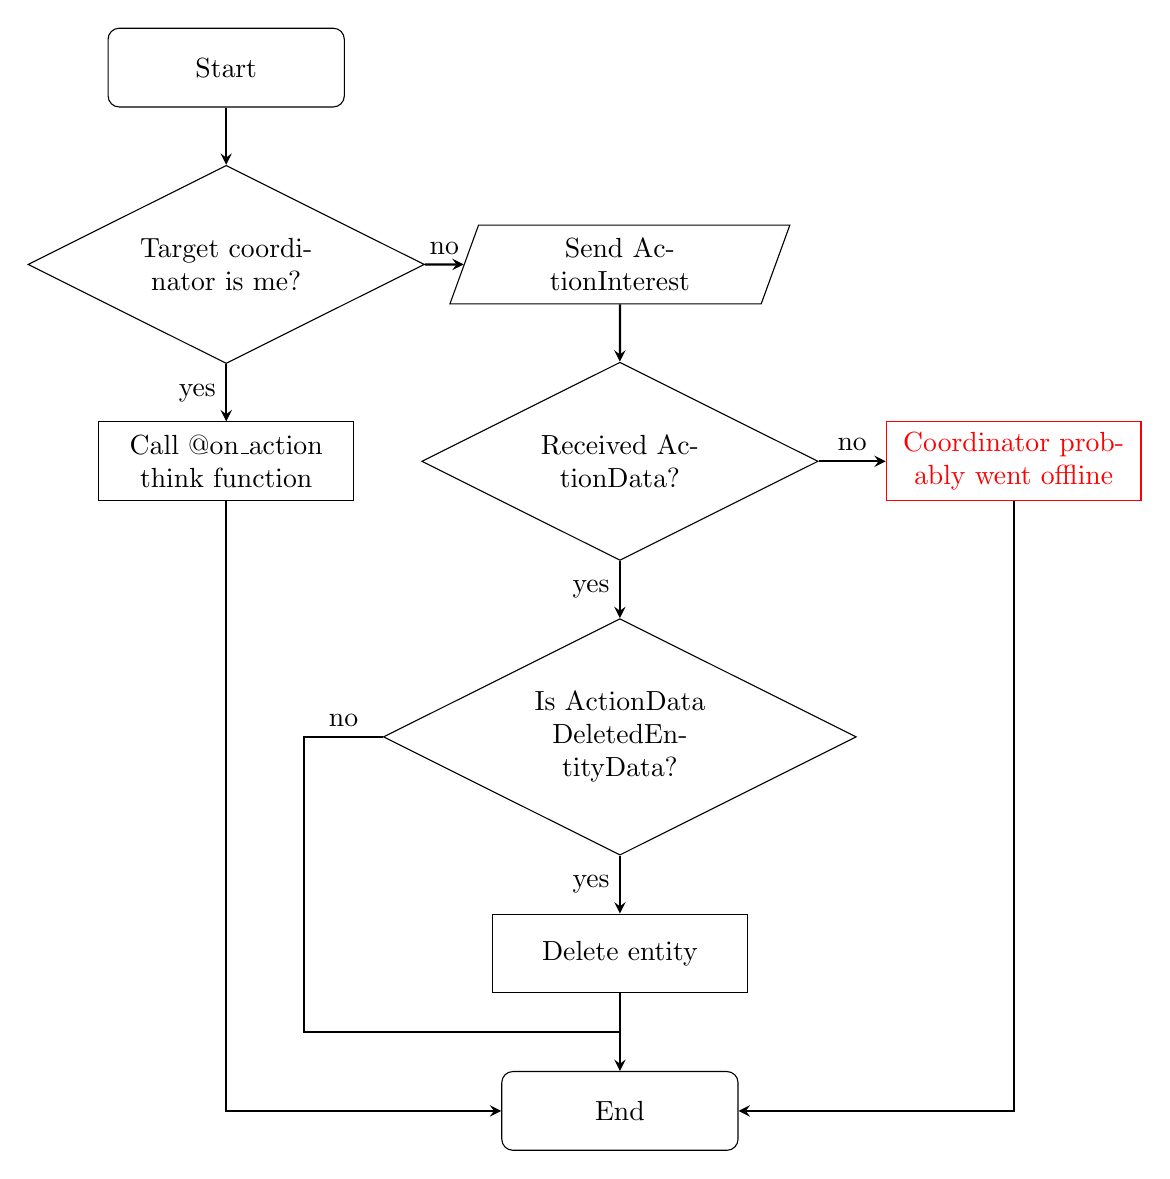
\begin{tikzpicture}[node distance=2cm]
  \node (start) [startstop] {Start};
  \node (dec1) [decision, below of=start, yshift=-0.5cm] {Target coordinator is me?};
  \node (pro1) [process, below of=dec1, yshift=-0.5cm] {Call @on\_action think function};
  \node (out1) [io, right of=dec1, xshift=3cm] {Send ActionInterest};
  \node (dec2) [decision, below of=out1, yshift=-0.5cm] {Received ActionData?};
  \node (dec3) [decision, below of=dec2, yshift=-1.5cm] {Is ActionData DeletedEntityData?};
  \node (pro2) [process, below of=dec3, yshift=-0.75cm] {Delete entity};
  \node (pro3) [process, red, right of=dec2, xshift=3cm] {Coordinator probably went offline};
  \node (stop) [startstop, below of=pro2] {End};

  \draw [arrow] (start) -- (dec1);
  \draw [arrow] (dec1) -- node[anchor=east] {yes} (pro1);
  \draw [arrow] (pro1) |- (stop);
  \draw [arrow] (dec1) -- node[anchor=south] {no} (out1);
  \draw [arrow] (out1) -- (dec2);
  \draw [arrow] (dec2) -- node[anchor=east] {yes} (dec3);
  \draw [arrow] (dec2) -- node[anchor=south] {no} (pro3);
  \draw [arrow] (dec3) -- node[anchor=east] {yes} (pro2);
  \draw [arrow] (pro2) -- coordinate (aux) (stop);
  \draw [arrow] (pro3) |- (stop);
  \draw [line] (dec3.west) -- node[anchor=south] {no} ++ (-1,0) |- (aux);
\end{tikzpicture}


\subsection{From coordinators}
\subsubsection{General handling process}
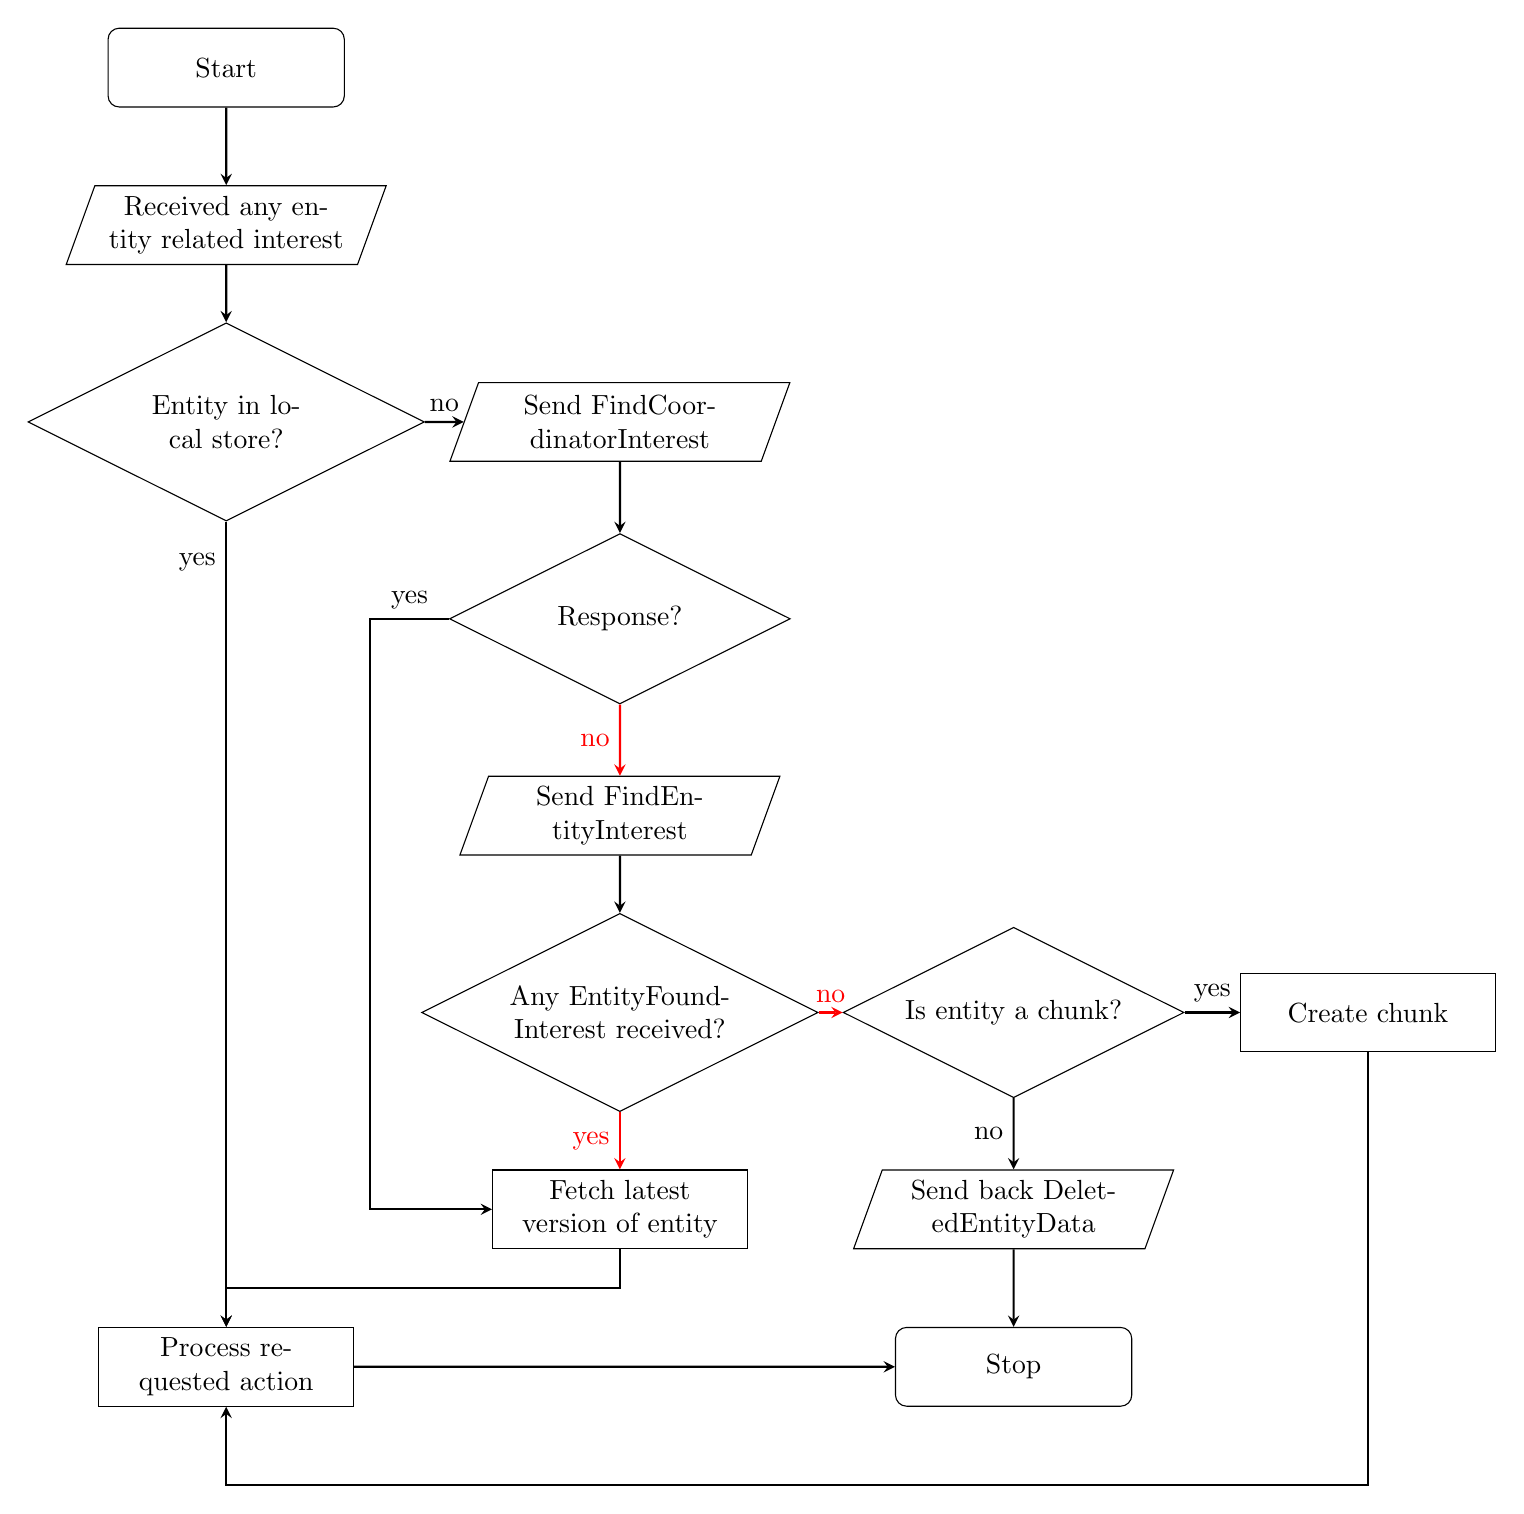
\begin{tikzpicture}[node distance=2cm]
  \node (start) [startstop] {Start};
  \node (in1) [io, below of=start] {Received any entity related interest};
  \node (dec1) [decision, below of=in1, yshift=-0.5cm] {Entity in local store?};

  \node (out1) [io, right of=dec1, xshift=3cm] {Send FindCoordinatorInterest};
  \node (dec2) [decision, below of=out1, yshift=-0.5cm] {Response?};

  \node (out2) [io, below of=dec2, yshift=-0.5cm] {Send FindEntityInterest};
  \node (dec3) [decision, below of=out2, yshift=-0.5cm] {Any EntityFoundInterest received?};
  \node (pro2) [process, below of=dec3, yshift=-0.5cm] {Fetch latest version of entity};

  \node (dec4) [decision, right of=dec3, xshift=3cm] {Is entity a chunk?};
  \node (pro3) [process, right of=dec4, xshift=2.5cm] {Create chunk};
  \node (out3) [io, below of=dec4, yshift=-0.5cm] {Send back DeletedEntityData};

  \node (stop) [startstop, below of=out3] {Stop};
  \node (pro1) [process, below of=dec1, yshift=-10cm] {Process requested action};

  \draw [arrow] (start) -- (in1);
  \draw [arrow] (in1) -- (dec1);
  \draw [arrow] (dec1) -- node[pos=0.05, anchor=east] {yes} (pro1);
  \draw [arrow] (pro1) -- (stop);

  \draw [arrow] (dec1) -- node[anchor=south] {no} (out1);
  \draw [arrow] (out1) -- (dec2);
  \draw [red,arrow] (dec2) -- node[anchor=east] {no} (out2);
  \draw [arrow] (dec2.west) -- node[anchor=south] {yes} ++ (-1,0) |- (pro2);

  \draw [arrow] (out2) -- (dec3);
  \draw [red,arrow] (dec3) -- node[anchor=east] {yes} (pro2);
  \draw [red,arrow] (dec3) -- node[anchor=south] {no} (dec4);
  \draw [arrow] (dec4) -- node[anchor=south] {yes} (pro3);
  \draw [arrow] (dec4) -- node[anchor=east] {no} (out3);

  \draw [arrow] (out3) -- (stop);
  \draw [arrow] (pro3) -- ++ (0,-6) -| (pro1.south);
  \draw [arrow] (pro2)  -- ++ (0,-1) -| (pro1.north);
\end{tikzpicture}

\subsubsection{Receiving action}

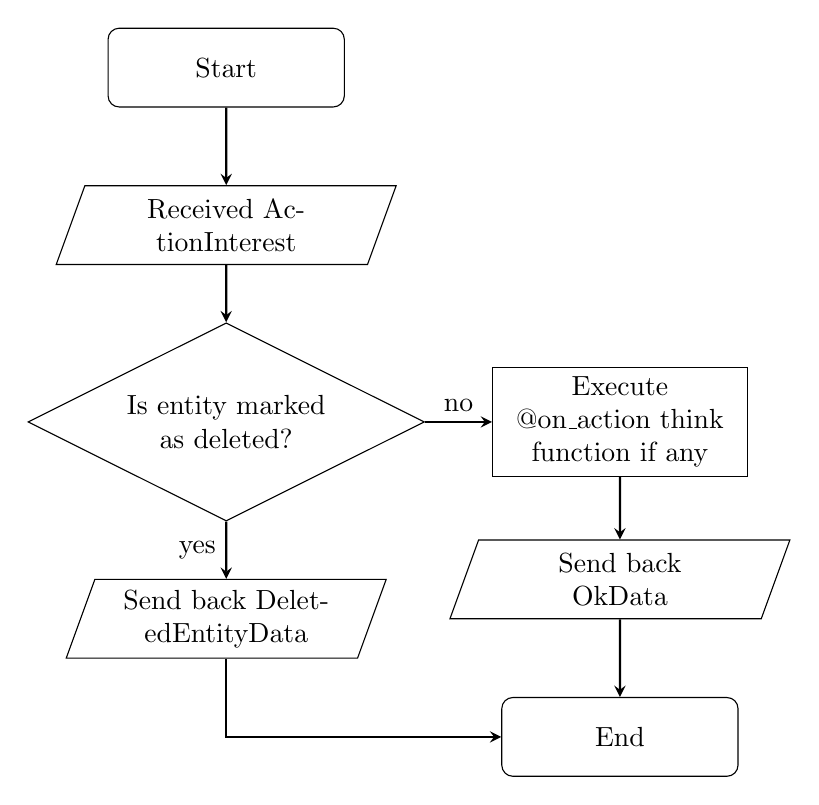
\begin{tikzpicture}[node distance=2cm]
  \node (start) [startstop] {Start};
  \node (in1) [io, below of=start] {Received ActionInterest};
  \node (dec1) [decision, below of=in1, yshift=-0.5cm] {Is entity marked as deleted?};
  \node (out1) [io, below of=dec1, yshift=-0.5cm] {Send back DeletedEntityData};
  \node (pro1) [process, right of=dec1, xshift=3cm] {Execute @on\_action think function if any};
  \node (out2) [io, below of=pro1] {Send back\\OkData};
  \node (stop) [startstop, below of=out2] {End};

  \draw [arrow] (start) -- (in1);
  \draw [arrow] (in1) -- (dec1);
  \draw [arrow] (dec1) -- node[anchor=east] {yes} (out1);
  \draw [arrow] (out1) |- (stop);
  \draw [arrow] (dec1) -- node[anchor=south] {no} (pro1);
  \draw [arrow] (pro1) -- (out2);
  \draw [arrow] (out2) -- (stop);
\end{tikzpicture}

\subsubsection{Sending objects}
\subsubsection{Sending updates}
When a object has been modified locally, the peer should send a UpdateData in response to the pending UpdateInterests to inform remote peer of the change in the state.


\end{document}
